\documentclass{sigchi}

% Use this command to override the default ACM copyright statement
% (e.g. for preprints).  Consult the conference website for the
% camera-ready copyright statement.

%% EXAMPLE BEGIN -- HOW TO OVERRIDE THE DEFAULT COPYRIGHT STRIP -- (July 22, 2013 - Paul Baumann)
\makeatletter
\def\@copyrightspace{\relax}
\makeatother
%% EXAMPLE END -- HOW TO OVERRIDE THE DEFAULT COPYRIGHT STRIP -- (July 22, 2013 - Paul Baumann)

% Arabic page numbers for submission.  Remove this line to eliminate
% page numbers for the camera ready copy
% \pagenumbering{arabic}

% Load basic packages
\usepackage{balance}  % to better equalize the last page
\usepackage{graphics} % for EPS, load graphicx instead 
\usepackage[T1]{fontenc}
\usepackage{txfonts}
\usepackage{mathptmx}
\usepackage[pdftex]{hyperref}
\usepackage{color}
\usepackage{booktabs}
\usepackage{textcomp}%
\usepackage{caption}
\usepackage{subcaption}
% Some optional stuff you might like/need.
\usepackage{microtype} % Improved Tracking and Kerning
% \usepackage[all]{hypcap}  % Fixes bug in hyperref caption linking
\usepackage{ccicons}  % Cite your images correctly!
% \usepackage[utf8]{inputenc} % for a UTF8 editor only

% If you want to use todo notes, marginpars etc. during creation of your draft document, you
% have to enable the "chi_draft" option for the document class. To do this, change the very first
% line to: "\documentclass[chi_draft]{sigchi}". You can then place todo notes by using the "\todo{...}"
% command. Make sure to disable the draft option again before submitting your final document.
\usepackage{todonotes}

% Paper metadata (use plain text, for PDF inclusion and later
% re-using, if desired).  Use \emtpyauthor when submitting for review
% so you remain anonymous.
\def\plaintitle{The Visualization Dashboard: A Browser-Based Tool for High-Dimensional Data Exploration}
\def\plainauthor{Geoffrey Roeder}
%\def\emptyauthor{}
\def\plainkeywords{Authors' choice; of terms; separated; by
  semicolons; include commas, within terms only; required.}
\def\plaingeneralterms{Documentation, Standardization}

% llt: Define a global style for URLs, rather that the default one
\makeatletter
\def\url@leostyle{%
  \@ifundefined{selectfont}{
    \def\UrlFont{\sf}
  }{
    \def\UrlFont{\small\bf\ttfamily}
  }}
\makeatother
\urlstyle{leo}

% To make various LaTeX processors do the right thing with page size.
\def\pprw{8.5in}
\def\pprh{11in}
\special{papersize=\pprw,\pprh}
\setlength{\paperwidth}{\pprw}
\setlength{\paperheight}{\pprh}
\setlength{\pdfpagewidth}{\pprw}
\setlength{\pdfpageheight}{\pprh}

% Make sure hyperref comes last of your loaded packages, to give it a
% fighting chance of not being over-written, since its job is to
% redefine many LaTeX commands.
\definecolor{linkColor}{RGB}{6,125,233}
\hypersetup{%
  pdftitle={\plaintitle},
% Use \plainauthor for final version.
%  pdfauthor={\plainauthor},
  pdfauthor={\plainauthor},
  pdfkeywords={\plainkeywords},
  bookmarksnumbered,
  pdfstartview={FitH},
  colorlinks,
  citecolor=black,
  filecolor=black,
  linkcolor=black,
  urlcolor=linkColor,
  breaklinks=true,
}

% create a shortcut to typeset table headings
% \newcommand\tabhead[1]{\small\textbf{#1}}

% End of preamble. Here it comes the document.
\begin{document}

\title{\plaintitle}

\numberofauthors{3}
\author{%
  \alignauthor{Geoffrey Roeder\\
    \affaddr{University of Toronto}\\
    \email{roeder@cs.toronto.edu}}\\
}

\maketitle%

\begin{abstract}
This research addresses a visualization gap between the needs of classical statistics and current practice in machine learning by introducing the Visualization Dashboard, a new tool for high dimensional data exploration. %
%
The Dashboard provides users with multiple state-of-the-art dimensionality reduction and clustering algorithms for exploring high-dimensional data. %
%
The Dashboard is designed for use in early phases of statistical and machine learning analyses, to assist in comprehending data for model exploration and feature extraction purposes. %
%
A review of prior work in this area shows it has focused primarily on synthetic data for pedagogical aims. %
%
Some prior work, hosted online, is integrated into the Dashboard to enrich user comprehension of parameter tuning in dimensionality reduction. %
%
Motivating design choices and functionality of the Dashboard are discussed in detail, followed by the results of a formative study and implications for information visualization theory.
\end{abstract}%
%
%
%
\section{Introduction}
%
%
%
Machine learning (ML) in practice follows a pipeline that begins with data cleaning and exploration and ends with a statistical model tailored to answer a particular question. % 
%
Information visualization can help a practitioner with this pipeline by providing valuable visualizations of high-dimensional data to aid in the formation of models that are effective for the task at hand. % 
%
Particular challenges in ML make existing tools inadequate. % 
%
Unlike data collected from carefully designed statistical experiments, the data handled in ML is often collected as a by-product of some other business process, such as the scrolling, clicking, and purchase behaviour of customers while browsing a retail website. % 
%
The features of such datasets are often redundant, and so they exhibit high statistical correlation with each other. % 
%
Correlated features reduce the efficacy of data mining techniques like generalized linear models by increasing the variance in the estimated model coefficients, leading to greater uncertainty in the model outputs. % 
%
Moreover, extra uninformative dimensions make the data exploration stage of the ML pipeline very challenging, because there exists no principled way of choosing which of the many dimensions to visualize for an arbitrary dataset. % 
%
\\\\
%
Visualizing data for exploratory purposes is a crucial step in an analysis that motivates the rest of the study, often suggesting a model class or a feature transform. %
%
Classical statistics has some tools to offer, like a matrix-style pairwise scatter plot showing how each pair of feature changes with respect to every other, accessible through the \texttt{pairs} function in the R programming language. % 
%
Such visualizations are instrumental in helping a practitioner choose the right features for a generalized linear model. % 
%
After perhaps nine dimensions, though, these plots become difficult to read and interpret. % 
New visualization tools are needed in the ML pipeline to help practitioners deal with the expanding ambition and data scale of the methods. %
%
\\\\
%
This project addresses the following research question: can a simple-to-use, automated dimensionality reduction and data-cluster tool improve the workflow of ML researchers during the model exploration phase of their analysis? % 
%
The motivation for this study stems from the author's personal experience working with a team of statisticians and mathematicians at an industry mathematical modelling workshop. %
%
The assigned task was to predict the output of an industrial fusion reactor using a subsample of 2 terabytes of time-series data. % 
%
The greatest bottleneck and most time consuming task was to discover an effective visualization of the data that revealed sufficient structure for the team to exploit to build a useful, interpretable predictive model.%
%
\\\\%
%
\begin{figure}
  \centering
  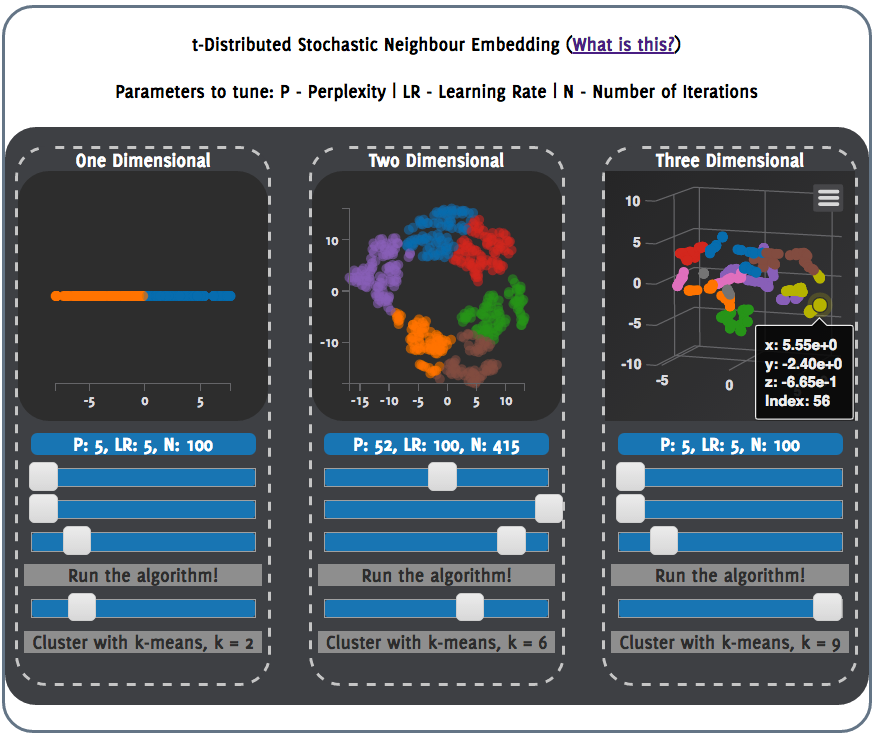
\includegraphics[width=.99\columnwidth]{figures/main_populated}
  \caption{Interface widget from the Visualization Dashboard populated with example data.}~\label{fig:figure1}
\end{figure}
%
Concretely, the research contribution is a high-dimensional data visualization dashboard (referred to as the \textit{Visualization Dashboard} in the remainder). % 
%
The Visualization Dashboard (see Figure 1) is a web application developed using the D3.js \cite{d3js} and Highcharts libraries in Javascript. %
%
The Visualization Dashboard allows users to easily load data from a locally-hosted file and to generate multiple reduced-dimensionality views on a raw dataset. % 
%
The views may then be clustered using the k-means centroid-based clustering (Hartigan \& Wong 1979) in order to reveal groups of related points. % 
%
The interface provides sliders for adaptively adjusting the parameters, and a button to re-run each algorithm with the new settings. % 
%
State-of-the-art dimensionality reduction techniques like t-Distributed Stochastic Neighbour Embedding (tSNE) \cite{maaten2008visualizing} require careful tuning of parameters to find useful results. % 
%
The Visualization Dashboard facilitates this tuning through the updatable views and sliders, and provides independent viewing panes for each of the three visualizable reductions (one, two, or three dimensions) and each of the algorithms currently implemented. % 
%
This allows a researcher to experiment and iterate quickly over different visualizations of a subsampled version of the dataset.% 
%
\\\\
%
After a review of recent work related to the Visualization Dashboard, the interface design will be presented in detail. Next, the results of a formative study are presented, followed by a discussion of implications this research has for information visualization theory in terms of the widely-used Data Space Model \cite{chi1999framework}.
%
%
%
\section{Background and Previous Work}
%
%
%
To the best of the author's knowledge, the Visualization Dashboard is the first interactive dimensionality reduction and clustering web application that presents different views of a dataset for data exploration. %
%
Common tools and software frameworks used for such purposes, like or \texttt{RStudio}, \texttt{Matlab}, or \texttt{Python}, require extensive knowledge of the particularities of the languages. %
%
The software package \texttt{Tableau} \cite{tableau} is closest in intention to the Visualization Dashboard. %
\texttt{Tableau} is a commercial software tool with a simple interface that can generate many different visualizations, intended for business applications. %
% http://www.tableau.com/learn/whitepapers/using-r-and-tableau
% https://www.r-bloggers.com/dream-team-combining-tableau-and-r/
For more advanced statistical techniques like dimensionality reduction, though, \texttt{Tableau} relies on integration with the R programming language. %
%
In contrast, the Visualization Dashboard encapsulates the statistical expertise needed to program an advanced algorithm by exposing only sliders and the algorithm output as a scatter plot. %
%
\\\\
%
There have been a number of recent research contributions that attempt to achieve a similar level of technical encapsulation for ML, and we review these in this section. %
%
%
\subsection{Visualizations to Support Machine Learning}
%
%
EnsembleMatrix\cite{talbot2009ensemblematrix} is a visualization tool designed to assist non-experts in ML in the task of combining independently-trained classifiers into the best performing ensemble%
%
\footnote{An ensemble classifier aggregates the output of a set of classifiers to make a final classification decision through majority voting, or a the highest probability class out of a weighted combination of the class-membership probabilities contributed by each component classifier.}. %
%
EnsembleMatrix presents a confusion matrix%
%
\footnote{A confusion matrix displays the number of classification decisions for each class label in a matrix. The true class label is the row label, and the predicted class label is the column label. A perfect classifier has no entries in the off-diagonal of the matrix.}, %
%
coloured as a heat-map as its central visualization. %
%
Users are given two interface widgets: (1) a polygon and brush tool that determines the weighting of each classifier by the position of the brush, and (2) the ability to partition the data by labels by clicking on the central confusion matrix visualization and apply a custom weighting scheme on that partition. %
%
Control point (1) allows a user to upweight classifiers that perform well on regions of the class space that have been isolated by control point (2). %
%
The combination of (1) and (2) allows a user to recursively identify areas of weakness in the ensemble classifier apply custom weighting schemes to strength the performance. %
%
Each change results in an immediate update of the confusion matrix. %
%
Such adaptive feedback allows fine-grained control over how the classifiers are combined into an ensemble. %
\\\\
A user study of the interface demonstrated that non-expert users were able to achieve state-of-the-art performance on an image classification task \cite{talbot2009ensemblematrix}. %
%
This validates the theory that well-designed visualization tools can give non-expert users access to very effective ML tools. %
%
Both the adaptive updates and the interface widget design concept were an inspiration for the Visualization Dashboard. %
%
EnsembleMatrix differs from the Visualization Dashboard because it intervenes in a later stage of the ML pipeline, after a group of models has already been constructed. %
%
The Visualization Interface presented in this paper intervenes in an earlier stage: determining what model class and what features can be modeled using the dataset. %
%
\\\\
%
ManiMatrix \cite{kapoor2010interactive} is another visualization that intervenes in the ML pipeline after a classifier has been trained. %
%
ManiMatrix presents users with a visualization of a cost function%
%
\footnote{A cost function is a mathematical tool from decision theory. It formalizes the natural idea that more costly mistakes should be avoided when doing classification (this is not a feature of the base mathematical formulation used in a classifier). %
Misclassifying a patient as suffering from the influenza virus when they are really suffering from a rhinovirus infection is not as serious as misclassifying skin cancer as a regular freckle. %
A cost function provides the mathematical object that tunes the decisions made by a classifier, allowing a statistician to minimize the risk of the most serious errors.}, %
%
a confusion matrix, and the decision boundaries generated by a classifier%
%
\footnote{A decision boundary is a region of the data space in which any point that falls in the region is classified identically. This is commonly visualized by colouring entire decision regions uniformly in a scatter plot of the points.}. %
%
ManiMatrix provides an interface widget that allows a user to change the cost function, represented as a matrix, up or down for each class. %
%
Every change triggers a fast update of the classification algorithm. %
%
This is reflected immediately in changes to the confusion matrix and decision boundary visualizations. %
%
\\\\
%
In a user study, \cite{kapoor2010interactive} found that their system allowed users to quickly and effectively tailor standard algorithms to problems with a complex cost and penalty structure. %
%
Their work demonstrates the gains that information visualization can offer ML practitioners by encapsulating algorithmic updates within adaptive displays and intuitive interface components. %
%
Such an interface allows users to avoid the expertise required (or, given the expertise, taxing work of) recalculating the model and re-running, re-visualizing the analysis scripts. %
%
The Visualization Dashboard works to provide the same encapsulation by hiding the unimportant details behind an effective user interface. %
%
ManiMatrix differs from the Visualization Dashboard differs in the same way as EnsembleMatrix: the intervention in the ML pipeline by ManiMatrix occurs after the difficult work of deciding on and training a model has been completed.%
%
%
\subsection{Visualizations to Teach Machine Learning}
%
%
Another set of research contributions, closer in technical framework to the Visualization Dashboard, have been developed recently to help teach complex ML concepts.
%
\\\\%
%
The architecture of a trained Convolutional Neural Network (CNN)%
%
\footnote{Neural networks are represented in ML as node-link diagrams because their mathematical structure corresponds precisely to a directed graph in which each input feature is a top-level node with no incoming edges, and each output features is a leaf node with no outgoing edges.} %
%
is visualized by \cite{harley2015interactive}. %
%
The network is trained to recognize the digit class of a handwritten digit. %
%
The goal of the interface is to enhance a user's understanding of CNNs in general and how they classify inputs. %
%
This is acheived by showing what parts of the network are most active during a classification decision. %
%
Users view a three-dimensional representation of the entire network, with a pane for drawing new digits with the mouse cursor. %
%
After entering a digit, users can move around the network structure in three dimensions using the interface %
%
Playing with this dynamic interface can help a user see what sorts of errors the network is prone to make, and can give a sense of how the network recognizes a given number. %
%
\\\\
%
Although a valuable learning tool to help users familiarize themselves with CNNs, the Node-Link visualization does not have any immediate applications for tuning or improving actual CNN models for image recognition. %
%
As of writing, practical neural architectures for image recognition are non-trivially more complex than the network visualized in \cite{harley2015interactive}, with many orders of magnitude more parameters and layers. %
%
In the image recognition community, this trend of increasing complexity is expected to continue. %
%
Nevertheless, \cite{harley2015interactive} is an important first step in the direction of visualizing complex neural architectures. %
%
Its use of three-dimensions in particular highlight the desire for better and more intuitive visualization methods in ML to aid practitioners in understanding and using models.%
%
\\\\
%
A few recently developed online teaching tools are similar in technology to the Visualization Dashboard. %
%
Setosa.io's Explained Visually \cite{setosaPCA} project demonstrates the Principal Component Analysis (PCA) dimensionality reduction algorithm \cite{jolliffe2002principal} using both a toy example and a real dataset. %
%
PCA finds orthogonal directions of greatest variance in a dataset, and then projects the data points onto as many or as few of those directions as desired, as a way of eliminating redundant or noisy information. %
%
The reduced dimensions are a linear function of the original dimensions, and so it is possible to gain intuition into how those original dimensions influence the new positions of the point.
%
In the Setosa.io interface, users can click and drag points displayed on a scatter plot to see how changing the location of inputs influences the projection onto 1 or 2 dimensions. %
%
This interactivity can help make the algorithm intuitive to a user, and aid in the interpretation of the results from a real dataset. %
%
\\\\
%
Similarly, the Google Brain research group released a set of visualizations \cite{wattenberg2016how} to help analysts understand how tuning particular parameters%
%
\footnote{Sometimes, the tunable components of tSNE are called \textit{hyperparameters} to emphasize their role in determining other parameters at a lower hierarchical level of the algorithm.} affects the output of tSNE \cite{maaten2008visualizing}. %
%
tSNE is the most complex algorithm included in the Visualization Dashboard. %
%
It is one of the most popular%
%
\footnote{In the eight years since its introduction to the time of writing, it has been cited 1973 times.} %
%
and widely used modern dimensionality reduction algorithms due to its ability to reproduce structure in high dimensions accurately in low dimensions \cite{maaten2008visualizing}. %
%
The tSNE visualizations in \cite{wattenberg2016how} provide toy examples of particular geometrical relationships among groups of data in high dimensional spaces, and shows how tSNE represents them in two dimensions given a judicious choice of parameters. %
%
\cite{wattenberg2016how} apply the same open-source library for tSNE, \cite{wattenberg2016how} as the Visualization Dashboard to generate the visualizations. %
%
The pedagogical value of \cite{wattenberg2016how} is very high, and it has been linked to in the Visualization Dashboard as a source of extra information to help users develop intuition about their data in the reduced dimensional space.%
%A recent innovation in t-SNE, one of the algorithms used for the Visualization Dashboard \cite{pezzotti2015approximated}, applies ideas from the field of Progressive Visual Analytics to make intermediate results of t-SNE useful. %
%
%t-SNE is a computationally intensive technique when applied to a large or complex dataset. %
%
%It can require intensive computation to reach optimal embeddings of high dimensional data in low dimensional spaces. %
%
%The work by \cite{pezzotti2015approximated} is an algorithmic and technical innovation that allows parital results from t-SNE to be viewed and adapted in real time to enable data exploration. %
%
%Interestingly, t-SNE is attempting to solve the same problem as the Visualization Dashboard, to help users identify clusters or patterns in data that can be used to generate novel hypothesis. %
%
%The key difference  is that the Visualization Dashboard renders a problem computationlly tractable by subsampling the data randomly in a way that preserves statistical properties, whereas \cite{pezzotti2015approximated} develop approximation methods that are computationally efficient in order to maintain the entire dataset. %
%
%\cite{pezzotti2015approximated} also apply cluster algorithms to help users see developing structures in the low-dimensional representation of the data, and additionally use a Magic Lens visualization to allow users to focus in on a region of interest. %
%
%[FOOTNOTE] a magic lense is a circular area that customizes the opacity of points so that only the points of interest are focused on.%
%

%\textbf{Previous Work in Statistics}

%Statisticians have been dealing with high dimensional datasets since the inception of the field. H

\section{Visualization Dashboard}
The Visualization Dashboard is a web application that runs locally in a user's browser. %
%
The central visualization component of the interface is shown in Figure 1. %
%
This section focuses on what a user is able to achieve with the interface, and the design choices that were made to facilitate this. %
%
\subsection{Technical Overview}
First, a brief description of the software used to develop the Visualization Dashboard is presented, intended to help other researchers select among the available libraries online. %
%
The highly developed state of open source ML Javascript libraries makes the development of experimental visualization software like the Visualization Dashboard much less resource intensive than it would have been in the recent past.%
%
\\\\
%
The dimensionality reduction algorithms were implemented using \texttt{ml-js} \cite{mljs} for PCA and general linear algebra, \texttt{tsnejs} \cite{tSNEJS} for tSNE, and \texttt{mdsjs} \cite{mdsjs} for the Multidimensional Scaling (MDS). %
%
Plotting functionality in 1D and 2D was implemented using D3.js \cite{d3js}, and 3D plotting was implemented using the Highcharts \cite{highcharts} framework. %
%
Automated data parsing was implemented using the \texttt{Papa Parse} \cite{papaparse} library.
%

\subsection{Design Overview}
The interface consists of a set of visual widgets like the one shown in Figure 1, stacked vertically in the window. %
%
The design choice of separated but visually similar widgets is intended to facilitate comparisons among the independent and equally valid views of a dataset. %
%
The name of the dimensionality reduction algorithm is written on the surrounding rectangle of each widget. %
%
\subsection{Data Loading}
The first interface component below the title is for loading data and labels into the application. %
%
\begin{figure}
  \centering
  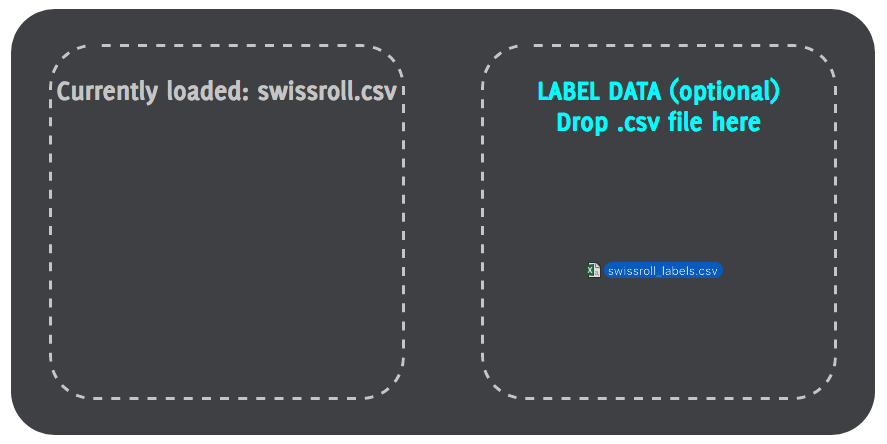
\includegraphics[width=.99\columnwidth]{figures/data_load}
  \caption{Data loading widget in the Visualization Dashboard}~\label{fig:figure2}
\end{figure}
%
Users are presented with two, equal-area dashed boxes with beveled edges inside of a surrounding visual region, darker than the background. %
%
When a user drags a file over the area, the text changes color from light grey to cyan to indicate the possibility of action. %
%
Once a user drops a file containing a dataset into the region, the text changes to "Currently loaded: Y" where Y is the name of the file. %
%
\\\\
%
This component of the interface has been designed with visual minimalism in mind by having a single point of focus that indicates an action is possible, or an action has been completed. %
%
These choices are meant to draw attention away from programmatic data loading issues and convey a sense of simplicity. %
%
The design is hoped to encourage experimentation by keeping the low-level details out of sight%
%
\footnote{The library chosen for data parsing, Papa Parse \cite{papaparse} can infer the format of the data from the first few lines (e.g. tab-separated, comma-separated, etc.). %
%
Although the prototype of the Visualization Dashboard recommends only comma-separated values, \cite{papaparse} can easily be extended to arbitrary data formats meaning that a user will not need to pay attention to how the data is formatted.}. %
%
The drag-and-drop choice is intended to encourage users to try loading in different datasets, and potentially different subsampled version of the dataset, which can be easily generated programmatically using command-line tools in Linux or generated graphically using Microsoft Excel. %
%
%
\subsection{1D and 2D Dimensionality Reduction}
%
%
Each dimensionality reduction widget like the one in Figure 1 initially contains three blank subdivisions that can be populated with scatter plots based on the reduced-dimensionality data (see Figure 1). %
%
Scatter plots were chosen for as the key visualization component of the Visualization Dashboard because they are a model-agnostic way of viewing data in 1, 2, or 3 dimensions. %
%
The three subdivisions are labelled above by the dimensionality of the data on display, in order to orient viewers in an information-dense visual field. %
%
Immediately below the viewing pane are the current values of tunable parameters for the algorithm, or other relevant information like the percentage of the original dataset's variance accounted for at the chosen level of reduced dimensionality in PCA. %
%
Depending on the complexity of the algorithm, more or fewer tunable parameters will be present. %
%
For example, with the tSNE algorithm, the parameters are Perplexity, Learning Rate, and Number of Iterations%
%
\footnote{See \cite{wattenberg2016how} for an overview of these parameters and how they influence the algorithm.} %
%
Each tunable parameters is controlled by a slider. %
%
Moving the sliders dynamically updates the values of the parameters. %
\\\\
%
Once settings for the parameters have been selected, the algorithm can be run using a button labelled "Run the algorithm!". %
%
As the mouse cursor moves over this button, the button inverts colors such that the dark text becomes light at the same time as the light background becomes dark. %
%
Such a dynamic inversion is a common way for web applications to indicate to a user that a region contains a latent possibility for action, and invites a mouse click. %
%
A second button in the subdivision is labelled "Cluster with K-means, k = Z" where Z is an integer between 1 and 10. %
%
A slider is present above this button, which dynamically changes the value of K. %
%
When no dataset is loaded, clicking these buttons has no effect.
%
%
\subsection{3D Dimensionality Exploration}%
%
%
\begin{figure}
\centering
\begin{subfigure}{.49\columnwidth}
  \centering
  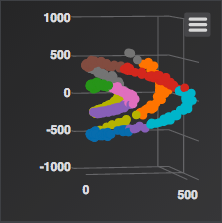
\includegraphics[width=.95\columnwidth]{figures/preclick3d}
  \caption{A 3D plot.}
\end{subfigure}%
\begin{subfigure}{.49\columnwidth}
  \centering
  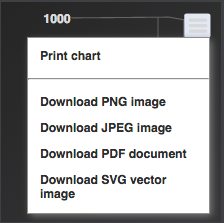
\includegraphics[width=.96\columnwidth]{figures/postclick3d}
  \caption{Options menu for saving figure.}
\end{subfigure}
\caption{Options for saving 3D visualizations.}
\label{fig:double}
\end{figure}%

The interface for 3D exploration provides more options due to the additional degree of complexity. %
%
Users can click and drag the viewport to rotate around the 3D structure and examine different points of view to look for interesting structures. %
%
Because the structures visible in 3D views are sensitive to the point of view, users are given the option of saving a particular view of the data in common image formats (see Figure 3). %
%
This functionality can be used to compare among views, to help an analyst decide what statistical model would, e.g., best separate out the classes or fit a curve for regression.%
%
\subsection{Clustering the Data with K-Means}
%
One clustering algorithm has been implemented in the prototype: K-Means \cite{hartigan1979algorithm}. %
%
K-Means was chosen because it is one of the most familiar, stable clustering algorithms, next to a perhaps too-simple density-based approach (e.g., \cite{ester1996density}).
%
Upon clustering the data, the different clusters are visualized by a change in point color. 
%
The K-Means cluster assignments correspond to a modelling assumption that the data was generated by sampling from a mixture of Normal distributions, where each component Gaussian is independent and has identical covariance. %
%
The means of the Normals correspond to the centers of the colored regions%
%
\footnote{Note that the colours themselves will sometimes change, but this is to be expected as the colours are arbitrarily assigned to the labels and carry no information other than group membership.}. %
%
This is a weaker assumption than it may appear at first, as the Normal distribution describes many dataset well as resulting from many different random effects combining together in a large sample. %
%
\subsection{Animations and Other Dynamic Components}
%
Two dynamic components of the interface convey key information about the dataset: tooltips appearing over individual points, and animations triggered when algorithms return new sets of reduced-dimensionality points. %
%
These dynamic components were chosen to help a user navigate an information-dense space of plots by providing informative and contextual cues as to the transformations taking place. %
%
\\\\
%
Tooltips can appear over any data point that is currently displayed in a viewing pane. %
%
The tooltip will appear on mouseover of the point and disappear when the mouse leaves that region. %
%
The tooltip provides the coordinates of the point and its row number in the raw dataset ("Index"). %
%
The coordinates are displayed so that the magnitude of difference between nearby points can be determined quantitatively, if desired. %
%
Unlike on a paper plot, it can be difficult to see exactly where a horizontal or vertical line through some point of interest intersects with the coordinate axes. %
%
A dynamic tooltip solves this problem cleanly. %
%
The alternative, displaying every value as a tuple next to the point, would be too visually cluttered for any dense set of points. %
%
\\\\
%
The index is provided because dimensionality reduction algorithms modify the actual coordinates of the points. %
%
This means that if a point was originally in six dimensions and is reduced to three, the three remaining dimensions are extremely unlikely to have the same value they began with after the algorithm has run. %
%
Hence, the index allows a user to investigate the points back in the original high-dimensional space to explore what correspondences might by causing their lower-dimensional distance. %
\\\\
%
Because some dimensionality reduction algorithms like tSNE are strongly influenced by their parameters settings, whenever the algorithm is run, an animation occurs in the visual display region. %
%
Whenever the "Run the algorithm!" button is clicked, the application calculates a new set of positions for the original data points. %
%
As soon the reduced-dimension dataset is available, all points currently on display inflate in size, then glide to their new positions over the period of one second.

The purpose of this animation is twofold. %
%
The first reason is to help a user track particular emerging clusters of interest. %
%
If a particular group of points appears together under one parameter setting, increasing or decreasing those parameters might cause the point cluster to either disperse, or contract even more tightly. %
%
Determining which behaviour has occurred can be a useful clue as to high dimensional structure in a dataset. %
%
The second, more speculative reason is to stoke the curiosity of a user about the changes that may occur next in a visualization as they vary parameters under some rationale. %
%
Attempting to find structure in high dimensional spaces can be frustrating due to the amount of creativity it requires for most people to imagine relationships in greater than three dimensions.
%
An interface with elements of play can encourage analysts to exploration of the possibilities in the dataset.%
%
\footnote{This is an independent research question that could be answered using the Visualization Dashboard with a suitably designed user study. For reasons of scope, I will leave this topic to another paper.} %
%
%
\subsection{Linking Out into the Online ML Community}
%
%
The ML community, like many other subdisciplines of the field of Computer Science, is strongly connected online. %
%
There are many excellent resources to help users understand dimensionality reduction algorithms (e.g. \cite{wattenberg2016how}, \cite{setosaPCA}. %
%
Even expert users can benefit from a review the effect of different parameters on how the algorithms behave. %
%
To make such review easy, links are provided next to the names of the algorithms that connect to useful resources. %
%
For example, next to the tSNE algorithm is a hyperlink to the recent Google Brain project \cite{wattenberg2016how} that explores how to tune the tSNE algorithm when the true high-dimensional dataset has a particular structure. %
%
\subsection{Case Study: Exploring Latent Structure in a Dataset}
%%
%
\begin{figure}
\centering
\begin{subfigure}{.49\columnwidth}
  \centering
  \includegraphics[width=.5\columnwidth]{figures/pca_3d_swiss}
  \caption{3D PCA.}
\end{subfigure}%
\begin{subfigure}{.49\columnwidth}
  \centering
  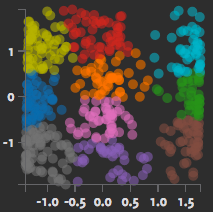
\includegraphics[width=.5\columnwidth]{figures/PCA_2d_roll}
  \caption{2D PCA.}
\end{subfigure}%
\\%
\begin{subfigure}{.49\columnwidth}
  \centering
  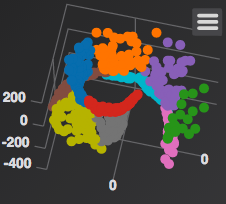
\includegraphics[width=.5\columnwidth]{figures/MDS_3d}
  \caption{3D MDS.}
\end{subfigure}%
\begin{subfigure}{.49\columnwidth}
  \centering
  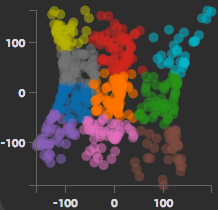
\includegraphics[width=.5\columnwidth]{figures/MDS_2d}
  \caption{2D MDS.}
\end{subfigure}\\%
\begin{subfigure}{.49\columnwidth}
  \centering
  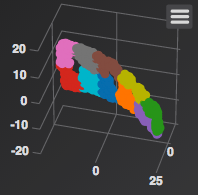
\includegraphics[width=.5\columnwidth]{figures/tSNE_3d}
  \caption{3D tSNE.}
\end{subfigure}%
\begin{subfigure}{.49\columnwidth}
  \centering
  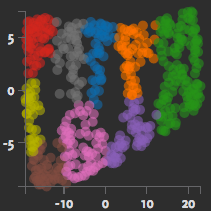
\includegraphics[width=.5\columnwidth]{figures/tSNE_2d}
  \caption{2D tSNE.}
\end{subfigure}
\caption{Swiss roll dataset after dimensionality reduction and parameter tuning.}
\label{fig:double}
\end{figure}%
%
This section provides a case study of how the Visualization Dashboard can be used to determine an appropriate model for a dataset. %
%
The dataset under analysis appears as a curved structure in 3D (see Figure 4). %
%
Although the structure in 3D has curvature, the points that lie on it are related to each other in a relevant way by only their positions on the "unrolled" roll. %
%
The structure is an example of a special kind of manifold in geometry, where the relevant distances (and hence similarities among points) can be best represented on a flat plane, but the plane is embedded in a higher dimensional space in which it is curved. %
%
\\\\
%
When reduced to 2D using the PCA algorithm (Figure 4b), it is not clear at all that the correct structure has been found. %
%
Indeed, by looking at the structure in 3D, it is clear that PCA has simply reduced the magnitude of the distances among points, but has kept the curvature of the embedding in 3D space intact. %
%
By comparing the 2D and 3D representations%
%
\footnote{Recall that due to the independent clustering algorithms run on the 2D and 3D representations, the colours will not match. They are presented here to help distinguish regions of the plots.}, %
%
it is evident that PCA has incorrectly collapsed the third dimension, squashing the cylinder into two dimensions. %
%
In such a representation, points which should be very far away from each other in the manifold (like points on the outside of opposite ends of the outside cylinder, corresponding to points in the green and dark blue regions of 4a) are now very close. %
%
\\\\
%
Similarly, MDS finds a different flattening of the space: the center of the roll is pinched inwards, but in 3D, it remains rolled. %
%%
In 2D, the same incorrect "squashing" phenomenon is observed. %
%
By playing around with the parameters of tSNE\footnote{To reproduce this result with the dataset swiss\_roll\_pi.csv (email author for access), set LR to 100, P to 50, and N to 500.}, %
however, we can discover exactly the structure we would expect to find in the synthetic dataset. %
%
This shows that tSNE discovers a lower dimensional representation that ignores the curvature of the embedded manifold in 3D and represents the high-dimensional structure correctly, using only 2 dimensions. %
%
This information can be used by an analyst to choose a model that encodes the data using only 2 output dimensions.
%%
%
\section{Evaluation: Formative Study}
A formative study was conducted in the late stages of development, after a working prototype was completed. %
%
The study was an unstructured interview with one pilot participant, who was at the time a graduate student in the ML Group at the University of Toronto. %
%

The participant was informed that the interface was useful for ML practitioners to understand high dimensional data. %
%
Without further instruction, the participant was then shown the interface, and asked to explore its functionality. %
%
The participant inferred that a data file could be dropped into the application, and that the interface would react to the data file by showing different visualizations of it. %
%
This suggests that no major flaws exist in the design concept. %
%
\\\\
%
The participant was then given access to a data file and asked to use the interface to explore it. %
%
After loading the file in the interface, he successfully generated a number of different visualizations. %
%
One behaviour of note is that after the three-dimensional visualization was discovered, which allows rotation around the point cloud, the participant attempted to click and dragging the two and one dimensional visualizations in order to elicit a similar response from the view. %%
%
When asked about the behaviour, the participant commented that the ability to pan or zoom is necessary to understand a dataset under exploration. %
%
\\\\
%
A final noteworthy result came from a request by the participant who asked for a tabular view of the raw data itself that could be modified with extra synthetic data. %
%
The paricipant noted that this would be useful for understanding intuitively how the reduced-dimensional representations are formed. %
%
The formative study suggests that the interface is effective in allowing exploration and study of complex datasets. %
%
The kinds of visualizations and play allowed by the current interface could be fruitfully extended in future enhancements to the interface according to the suggestions given. %
%
These enhancements can be built into the existing framework in a straightforward manner, now that the core functionality has been developed. %
%
\section{Discussion and Future Work}%
%
\begin{figure*}
  \centering
  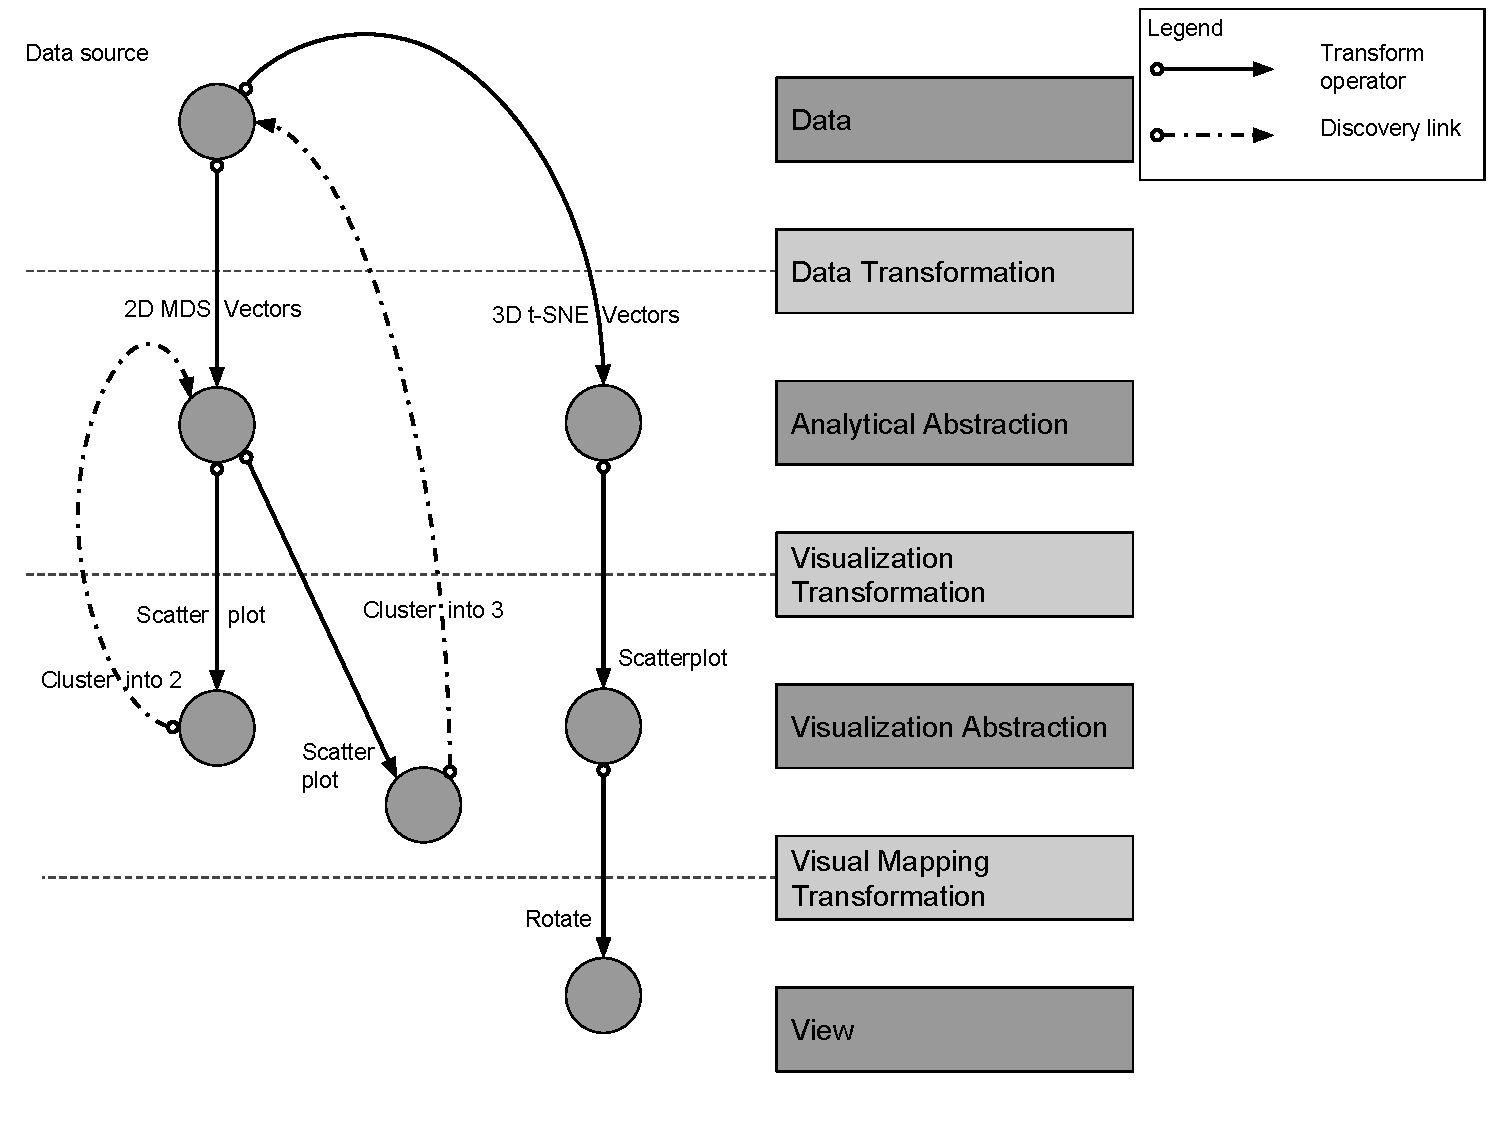
\includegraphics[width=2\columnwidth]{figures/extended}
  \caption{An extended Data Space Model that captures exploratory data visualizations}~\label{fig:figure2}
\end{figure*}
%
Based on the formative study, the author concludes that the interface is ready for use as a research platform into high-dimensional visualization.%
%
Moreover, the process of producing this interface has provided an opportunity to consider how current theoretical perspectives in the field of information visualization can be leveraged to understand the Visualization Dashboard. %
%
Chi's Data Space Model of information visualization is useful here as a model of the user interacting with the Visualization Dashboard.%
%
Chi's model is designed to capture the process of analysis that yields multiple visualization of a dataset. %
%
Raw data is transformed through four stages: first to an analytical abstraction representing the data as some abstract data structure like a graph, tree, or vector, next to a visualization abstraction like a network diagram, point set, or surface, and finally to a view of the data that displays some salient features of interest. %
%
\\\\
%
Chi's model is an extension of Stuart Card's Information Visualization Pipeline that imagines an analyst proceeding through a single path from raw data to final view \cite{chi1999framework}. %
%
Chi's model extends Card's to allow multiple paths, some of which terminate before yielding a final visualization. %
%
The Visualization Dashboard motivates an extension to Chi's model that can capture the process by which a ML researcher learns about data using multiple, temporary visualizations. %
%
The extension involves the addition of backlinks from the visual abstraction layer in Chi's model to previous layers, effectively permitting cycles through the network (see Figure 5 for a simple example). %
%
The backlinks represent "discovery links", where the current visual abstraction has given some useful information that motivates a new branch from an earlier node in the path.
%
Such an extended Data Space Model tracks the heuristic steps that an analyst takes in discovering relevant structure by tracing the links among the diagrams. %
%
This model could serve as a map for other researchers looking at similarly data to help guide their exploration of the high dimensional space, or simply provide a slightly richer framework for analyzing visualization systems. %
%
The scope of the present paper does not include a strong theoretical aims, so a further development of this contribution will be left to future projects. %
%
%
%
\section{Conclusion}%
%
%
%
This paper has introduced the Visualization Dashboard, a high-dimensional data exploration tool designed to support ML researchers in the early phase of model building. Design choices have been described and explored in the context of the intended use of the tool. A formative study has shown that the tool is ready to be used as a platform to answer research questions, and a novel extension to the Data Space Model has been proposed to describe the use of visualizations by a user of the Visualization Dashboard.
%

% References must be the same font size as other body text.
\bibliographystyle{SIGCHI-Reference-Format}
\bibliography{sample}

\end{document}

%%% Local Variables:
%%% mode: latex
%%% TeX-master: t
%%% End:
